
\section{Network Architecture}
\label{sec:arch}

%An in-depth examination of architectures via trial and error is left  future 

We begin with the notion that the discretization procedure outlined in Section \ref{sec:simulation} produces $25\times 25$ ``transverse-energy-scale'' images in one channel -- a High Energy Physics analogue of a grayscale image. We note that the images we work with are \emph{sparse} -- roughly 12\% of pixels are active on average. Future work can build on efficient techniques for exploiting the sparse nature of these images. However, since speed is not our driving force in this work, we used convolution implementations defined for dense inputs.  We also study fully connected MaxOut networks~\cite{maxout:goodfellow}.  Other architectures were also studied, such as Stack Denoising Autoencoders~\cite{SDAE}, and multi-layer fully connected networks with various activation functions, but found that convolution and MaxOut networks were the most performant.

As a brief aside, we discuss some of the key neural network concepts which are used in the following section to describe our network architectures.  Fully connected (FC) layers take all features as input.  Convolution networks utilize convolution filters (or kernels) which operate on a small $n\times n$ patch of the input image.  For instance, a $3\times3$ filter takes as input a $3\times3$ (horizontal $\times$ vertical) patch of pixels and applies a linear weighting to these pixels $z = \sum_{i,j=1}^{3} x_{ij}W_{ij} + b_{ij}$, where $x_{ij}$ is the input image patch, thus producing an output which can be considered as centered on that patch.  Each filter is convolved with the input image, in that the filter is applied to a given input patch and then moved horizontally and/or vertically to a new input patch on which the filter is applied.  By scanning over the entire image in this way, a the filter is convolved with the input, producing a convolved output.  A non-linear activation function is typically applied to these convolution outputs, for which we use the Rectified Linear Unit (ReLU)~\cite{RELU} which takes an input $z$ and outputs $\max\{0,z\}$. ReLU's have been found to improve network training time, whilst having enough non-linear behavior to not degrade network performance.    The MaxOut activation unit takes an input vector $x$ and computes $k$ linear weightings $z_{j} = \sum_{i} x_{i} W_{ij} + b_{j}$, where $j\in \{1...k\}$, and  outputs $\max_{j\in [1,k]}\ z_{j}$.  

\subsection{Architectural Selection} % (fold)
\label{ssub:architectural_selection}
For the MaxOut architecture, we utilize two FC layers with MaxOut activation (the first with 256 units, the second with 128 units, both of which have 5 piecewise components in the MaxOut-operation), followed by two FC layers with ReLU activations (the first with 64 units, the second with 25 units), followed by a FC sigmoid layer for classification. We found that the He-uniform initialization~\cite{HE_initialization} for the initial MaxOut layer weights was needed in order to train the network, which we suspect is due to the sparsity of the jet-image input. In cases where other initialization schemes were used, the networks often converged to very sub optimal solutions.  This network is trained (and evaluated) on un-normalized jet-images using the transverse energy for the pixel intensities

For the deep convolution networks, we use a convolutional architecture consisting of three sequential \texttt{[Conv + Max-Pool + Dropout]} units, followed by a local response normalization (LRN) layer~\cite{dropout:and:LRN}, followed by two fully connected, dense layers. We note that the convolutional layers used are so called ``full'' convolutions -- i.e., zero padding is added the the input pre-convolution. A conceptual visualization of the network architecture can be seen in Figure~\ref{fig:arch}. Our architecture can be succinctly written as:
\begin{equation}
  \mathtt{[Dropout \rightarrow Conv \rightarrow ReLU \rightarrow MaxPool] * 3 \rightarrow LRN \rightarrow [Dropout \rightarrow FC \rightarrow ReLU]  \rightarrow Dropout \rightarrow Sigmoid}.
\end{equation}

\begin{figure}[!htbp]
  \centering
  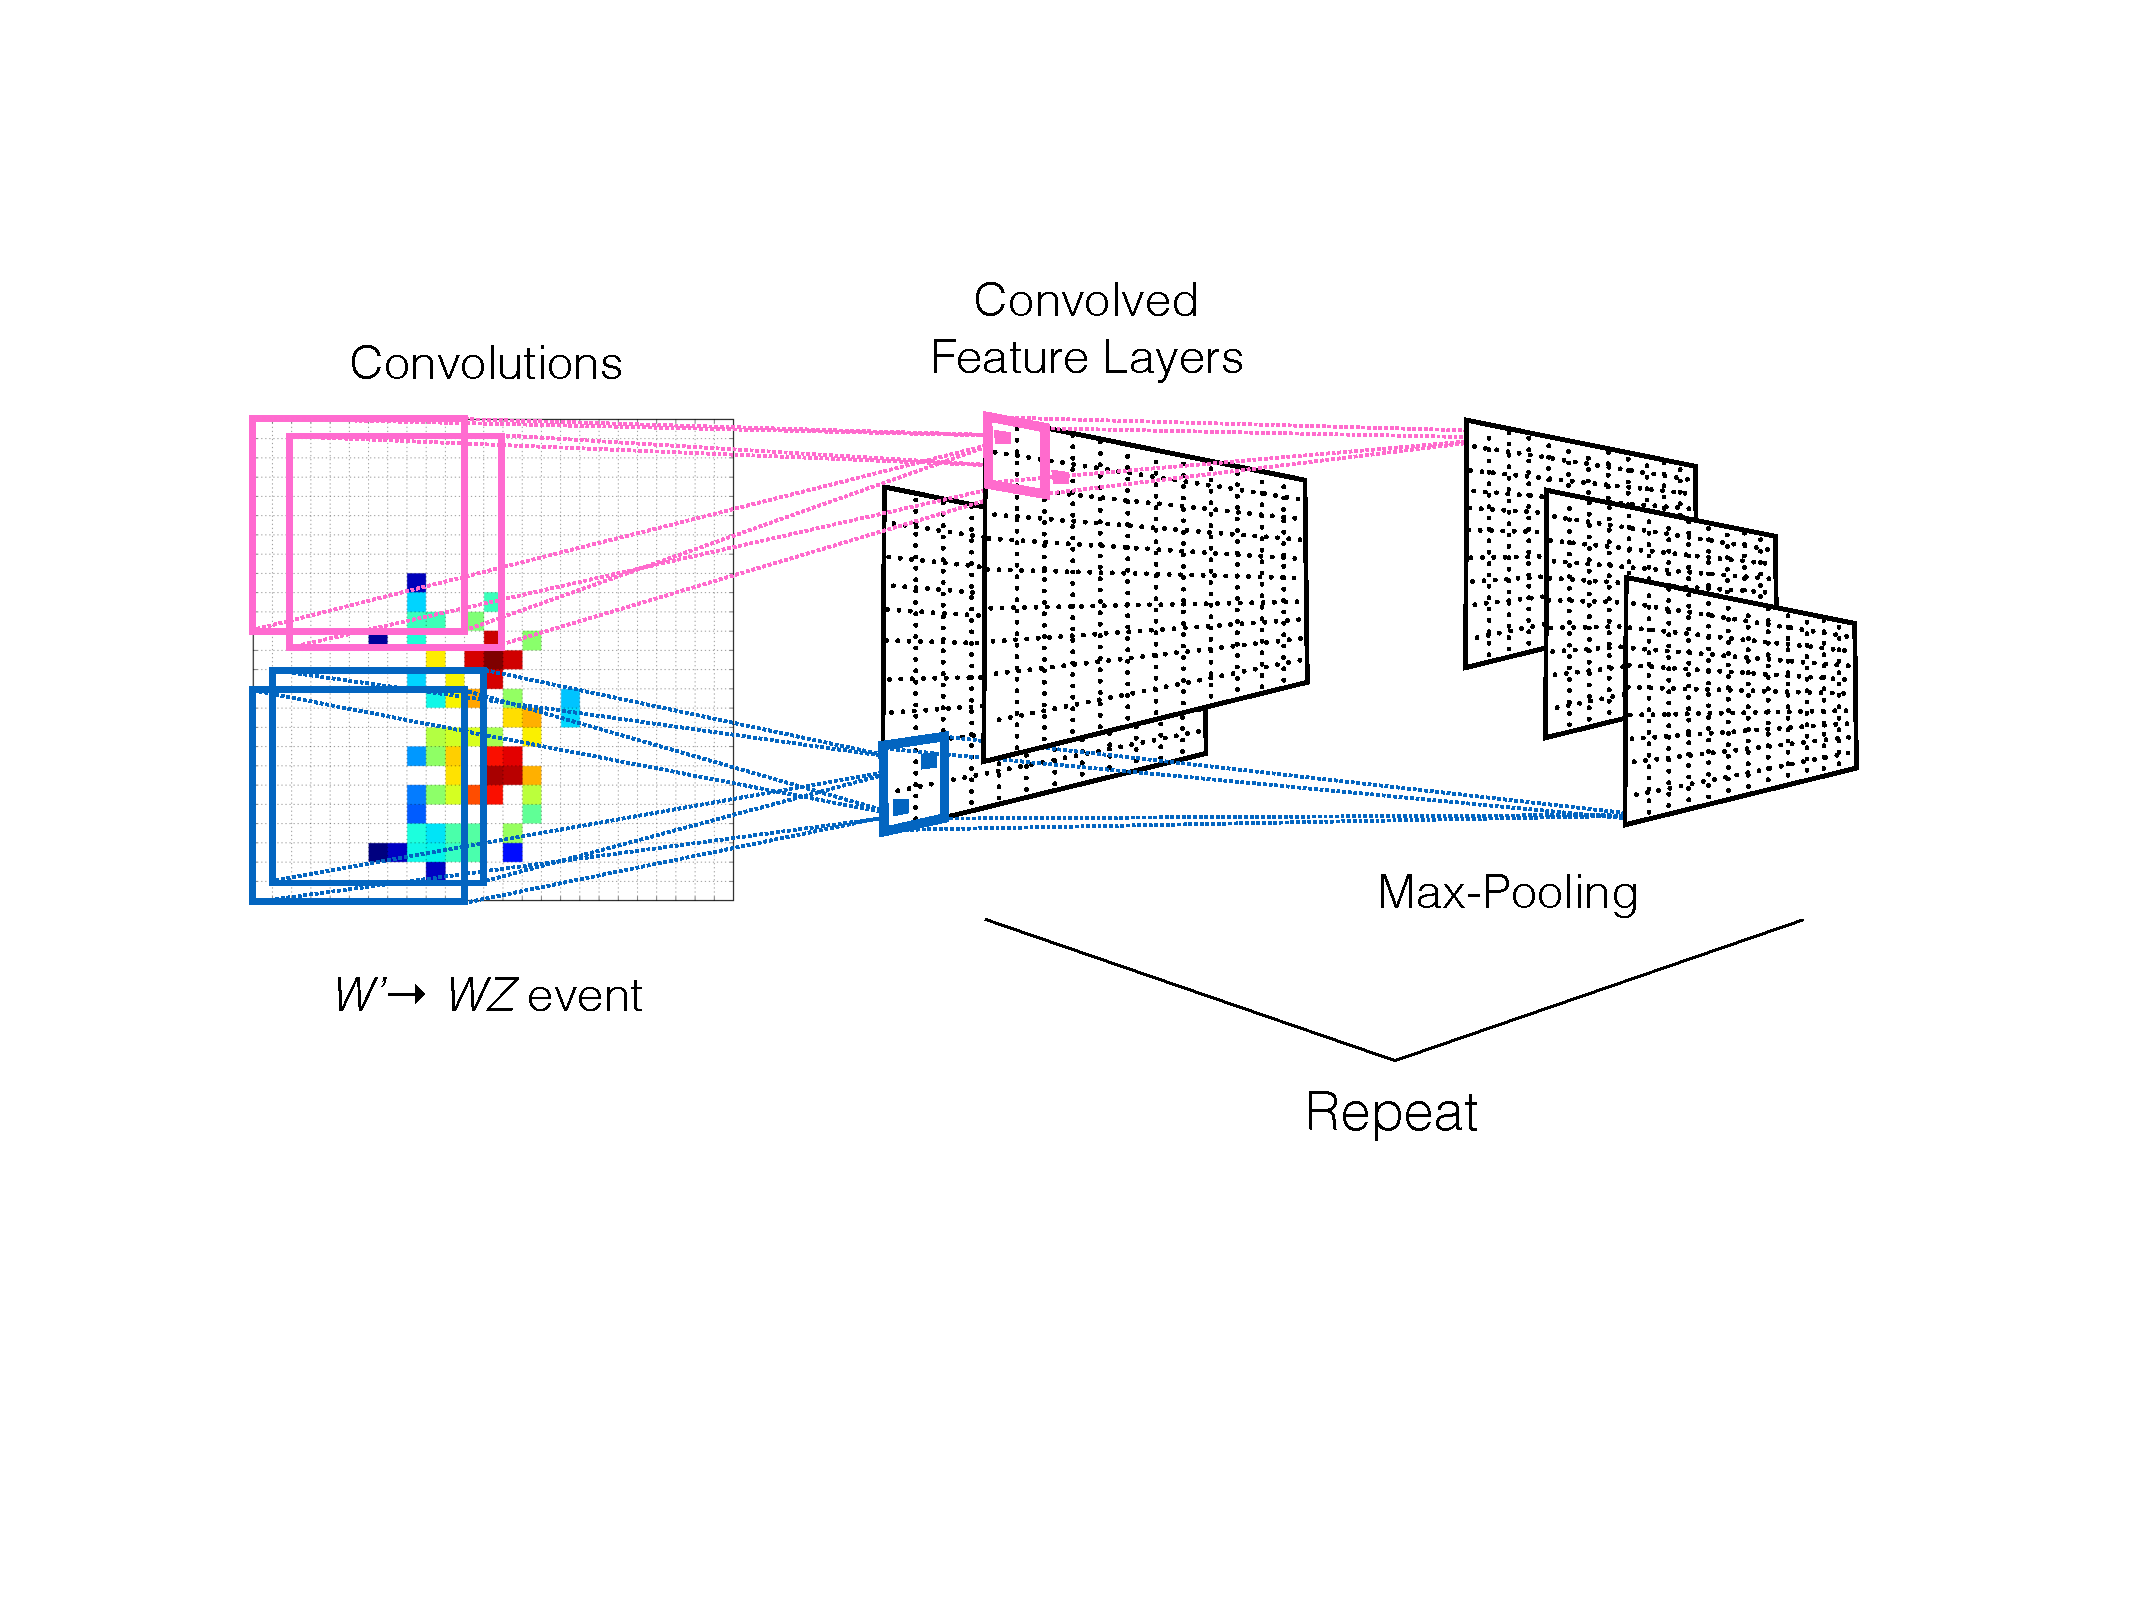
\includegraphics[width=0.75\textwidth]{figures/architecture.pdf}
  \caption{The convolution neural network concept as applied to jet-images.}
  \label{fig:arch}
\end{figure}

The convolution layers each utilize 32 feature maps, or filters, with filter sizes of $11\times 11$, $3\times 3$, and $3\times 3$ respectively.  All convolution layers are regularized with the $L^{2}$ weight matrix norm.  A down-sampling of $(2, 2)$, $(3, 3)$, and $(3, 3)$ is performed by the three max pooling layers, respectively.  A dropout~\cite{dropout:and:LRN} of 20\% is used before the first FC layer, and a dropout 10\% is used before the output layer.  The FC hidden layer consists of 64 units.

After early experiments with the standard $3\times 3$ filter size, we discovered significantly worse performance over a more basic MaxOut \cite{maxout:goodfellow} feedforward network. After further investigation into larger convolutional filter size, we discovered that larger-than-normal filters work well on our application. Though not common in the Deep Learning community, we hypothesize that this larger filter size is helpful when dealing with sparse structures in the input images. In Table~\ref{tab:kernelsize}, we show the optimal filter size of $11\times11$ while considering the metric outlined in Section~\ref{sec:studies}.

\begin{table}[h!]
  \centering
  \begin{tabular}{r|c}
    \bfseries Kernel size & \bfseries AUC \\ 
    \hline
    $(3 \times 3)$ Conv & 14.770 \\
    \hline
    $(4 \times 4)$ Conv & 12.452 \\
    \hline
    $(5 \times 5)$ Conv & 11.061 \\
    \hline
    $(7 \times 7)$ Conv & 13.308 \\
    \hline
    $(9 \times 9)$ Conv & 17.291 \\
    \hline
    $(11 \times 11)$ Conv & 20.286 \\
    \hline
    $(15 \times 15)$ Conv & 18.140 \\
  \end{tabular}
  \caption{First layer convolution size vs. performance}
  \label{tab:kernelsize}
\end{table}
% table

Two convolution networks, which differ in their pre-processing, are studied in this paper.  The first, which we refer to as the ConvNet, is trained (and evaluated) on un-normalized jet-images using the transverse energy for the pixel intensities.  The second, which we refer to as ConvNet-Norm, is trained (and evaluated) on $L^{2}$ normalized jet-images using the transverse-energy for the pixel intensities.  Examining the performance of both networks allows us to study the possible effects of the pre-processing.



% subsubsection architectural_selection (end)

\subsection{Implementation and Training} % (fold)
\label{ssub:implementation_and_training}

All Deep Learning experiments were conducted in Python with the Keras~\cite{Keras} Deep Learning library, utilizing NVIDIA C2070 graphics cards. One GPU was used per training, but several architectures were trained in parallel on different GPU's to optimize the performance of networks with different hyper-parameters.

We used 8 million training examples, with an additional 2 million validation samples for tuning the hyper-parameters, and 3 million testing samples.  Signal examples are weighted such that the total sum of weights is the same as the total number of background examples (as explained in Section~\ref{sec:simulation}).  These weights are used in the by the cost function in the training.  The networks were trained with the Adam~\cite{DBLP:journals/corr/KingmaB14} algorithm (Stochastic Gradient Descent with Nesterov Momentum~\cite{Nesterov:1983wy} was also examined, but did not provide performance gains).  The training consisted of 100 epochs, with a 10 epoch patience parameter on the increase in AUC between 0.2 and 0.8 on a validation set.  Batch sizes of 32 were used for the MaxOut network, while batch sizes of 96 were used for the convolution networks.

% subsubsection implementation_and_training (end)

